\documentclass{article}
\usepackage[utf8]{inputenc}
\usepackage{cite}
\usepackage{amsmath,amssymb,amsfonts}
\usepackage{graphicx}
\usepackage{textcomp}
\usepackage{xcolor}
\usepackage{booktabs}
\usepackage{multirow}
\usepackage{diagbox}
\usepackage{listings}
\usepackage{geometry}
\usepackage{verbatim}
\usepackage{subfigure}
\usepackage{abstract}
\usepackage{fancyhdr}
\usepackage{color}
\usepackage{float}
\usepackage{url}
\usepackage[colorlinks,linkcolor=blue,anchorcolor=blue,citecolor=red]{hyperref}
\usepackage{makecell}
\usepackage{indentfirst}
\setlength{\parindent}{2em}

\title{\textbf{The optimal choice of routing path\\Mobile Internet Homework1}}


\begin{document}
\maketitle

\begin{abstract}
The optimal choice of routing path. I use greedy algorithm to solve this problem. And in the paper, I will give an easy-to-understand proof.


\textit{Key Words: }Routing Path, Greedy Algorithm, Optimal Proof.
\end{abstract}


\section{Problem}
To focus more on the algorithm and method, I briefly summarize the description of the problem:

Considering there are n links between A and B, what we want to do is to find a method checking the the path between A and B with an optimal cost. We have the probability $p_i$ and the cost $c_i$ for each link $i$. 

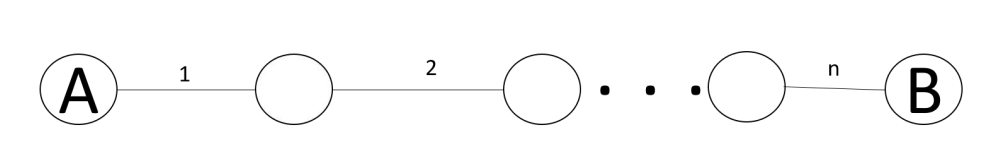
\includegraphics[scale=0.45]{1.png}

\section{Algorithm}
To solve this problem, I choose to use \textbf{greedy algorithm}. 

The detailed method shows as follow:

\begin{enumerate}
    \item Sort these links with the value $\frac{c_i}{1-p_i}$ as an ascending order.
    \item Check these links as the sorted order one by one.
\end{enumerate}

\textbf{By this algorithm, we can have an optimal cost.}

\section{Proof}
The following is the proof using exchange argument technique:

Considering there are two links $i$ and $j$, which have the property that $\frac{c_i}{1-p_i} \le \frac{c_j}{1-p_j}$.

From our algorithm, we will check $i^{th}$ path, then wo check $j^{th}$ path.

In the exchange argument technique, I will give the proof that if we check $j$ before $i$, we will introduce another cost.

\begin{center}\caption{\textbf{Probability and Cost Table}}
\begin{tabular}{|&|&|&|&|} 
\hline
Exist Condition& Probability & Cost for Optimal Method &Cost for Exchange Method \\ 
\hline
$i$ and $j$ both exist& $p_i  p_j$ & $c_i+c_j$ & $c_i+c_j$ \\ 
\hline
$i$ exists and $j$ not exists&  $p_i (1-p_j)$ & $c_i+c_j$&$c_j$ \\ 
\hline
$i$ not exists and $j$ exist&$(1-p_i)  p_j$ &  $c_i$ & $c_i+c_j$ \\ 
\hline
$i$ and $j$ both not exist& $(1-p_i)  (1-p_j)$ & $c_i$ & $c_j$ \\ 
\hline
\end{tabular}
\end{center}

Set $\Delta C$ as the extra cost from exchangement, then we can have the following expression:

\begin{equation}
    \Delta C = \sum Probability \cdot \Delta cost For Each Small Condtion
\end{equation}

Introducing the concreate value:
\begin{equation}
    \Delta C = \Delta C1+\Delta C2+\Delta C3+\Delta C4
\end{equation}

\begin{equation}
    \Delta C1 = p_i  p_j \cdot [(c_i+c_j) - (c_i+c_j)]
\end{equation}

\begin{equation}
    \Delta C2 = p_i (1-p_j) \cdot [(c_j) - (c_i+c_j)]
\end{equation}

\begin{equation}
    \Delta C3 = (1-p_i)  p_j \cdot [(c_i+c_j) - (c_i)]
\end{equation}

\begin{equation}
    \Delta C4 = (1-p_i)  (1-p_j) \cdot [(c_j) - (c_i)]
\end{equation}
                
\textbf{Finally}
\begin{equation}
    \Delta C = c_j(1-p_i)-c_i(1-p_i)
\end{equation}

\textbf{By Condition} $\frac{c_i}{1-p_i}\le\frac{c_j}{1-p_j}$, we have $\Delta C \ge 0$.

In this case, we can conclude that our optimal algorithm will not increase any cost comparing any other algorithm. It means it is the optimal algorithm.









\end{document}